\chapter{Implementation}\label{chp:implementation}

\section{Introduction}

An obstruction detector and a vanishing point detector are the two attempted implementations presented in this report. The obstruction detector uses stereo vision to perceive depth and distance to possible objects in the path of the robot. The vanishing point detector attempts to find a single vanishing point by detecting lines in the environment before selecting a vanishing point based on line intersections. 

\section{Vanishing Point Detection}

\subsection{Overview}

The goal of the vanishing point detector is to provide a setpoint for the robot to steer towards. In other words, steering towards a vanishing point is a good way to reach the end of a hallway or corridor. This was considered to be a good starting point, and possible expantions could be added later. Choosing a method as a basis for a vanishing point detector was not easy. The selected method should be simple, suitable for \gls{opencv} and not go too far beyond the prior knowledge of the author. Another important factor was that spending too much time on this implementation would come at the expense of the obstruction detector. A vanishing point detector method by D. Gerogiannis et. al. \cite{gerogiannisvp} showed promise as it was based on line detection, which has good support in OpenCV. The method in \cite{gerogiannisvp} appears to be suitable for structured environments with many straight lines, such as hallways, streets and corridors. The steps in the detection procedure are:

\begin{enumerate}
	\item Detect edges in the image, e.g. by using Canny edge detection.
	\item Detect line segments that may be used as vanishing lines based on edges found in step 1. Could be done with the Hough line transform.
	\item Filter the detected lines. This is done by modelling new lines by using the major axis of ellipses with very high eccentricity. The ellipses are generated by a split-and-merge algorithm. In short, it will merge similar line segments by assuming that their end points are collinear.
	\item Find line intersection points based on the new filtered lines. Each point is stored and assigned a weight.
	\item Find the vanishing point among the line intersections based on a voting scheme. 
\end{enumerate}

\subsection{Line Detection}

Line detection comprise step 1 and 2 from the list above. OpenCV comes with an implementation of the Canny edge detector ready for use. The detector returns a binary image of the detected edges. Edges are detected by convolving the input image with two kernels $G_x$ and $G_y$. The convolutions will indicate change gradients in the $x$ and $y$ directions which in turn will give the direction of a potential edge. Finally, the detector rejects or accepts potential edges based on two gradient thresholds. Gradients below the lower threshold are rejected, edges above the upper threshold are accepted, and edges between the thresholds are only accepted if their neighbouring gradients are above the upper threshold\cite{cannyedge}. 

\begin{wrapfigure}{r}{0.55\textwidth}
	\vspace{-10pt} % Remove exessive whitespace
	\centering
	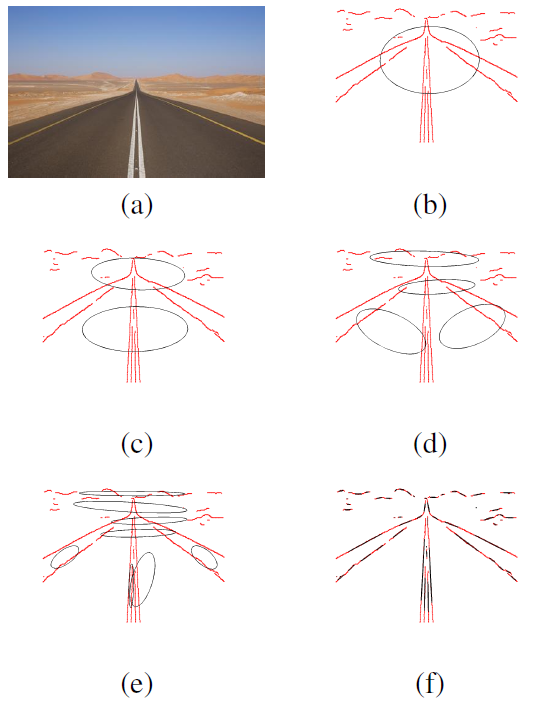
\includegraphics[width=0.6\textwidth]{GerogiannisLines}
	\caption{\label{fig:GerogiannisLines}Gerogiannis concept of representing lines by eccentric ellipses. This image is taken directly from \cite{gerogiannisvp}.}
	\vspace{-60pt} % Remove exessive whitespace
\end{wrapfigure}

At this point, we only have a simple binary image where edges are represented as white pixels on a black background. The next step is to interpret these edges as lines. Line detection is performed by using the probabilistic Hough line transform. This is an already implemented function, which takes in the edge image from the previous step, and return a set of point pairs representing line segments. The benefit of using the probabilistic detector is that it can perceive an edge with a discontinuity as a singe line. 

\subsection{Line Filtering}

Line filtering is performed by splitting and merging ellipses until their major axis represents a set of approximations to collinear points. The points is the set of points that define the previously detected line segments. This algorithm is called \gls{dsam}, and it is explained in another paper by D. Gerogiannis \cite{gerogiannisshape}. Line segments returned from the probabilistic Hough transform will often overlap or be very close to each other. The purpose of this step is to get a cleaner representation of the contours in the environment.

Figure \ref{fig:GerogiannisLines}, taken from \cite{gerogiannisvp}, illustrates the steps in the \gls{dsam} algorithm.

\subsection{Vanishing Point Detection}

\begin{wrapfigure}{r}{0.35\textwidth}
	\vspace{-10pt} % Remove exessive whitespace
	\centering
	\includegraphics[width=0.36\textwidth]{getVp}
	\caption{\label{fig:getVp}Two steps in \textit{getVanishingPoint()}.}
	\vspace{-60pt} % Remove exessive whitespace
\end{wrapfigure}


When the detected lines have been filtered and stored, they will be passed to the vanishing point detector in the function \textit{getVanishingPoint(lines)}. This function will perform two steps (figure \ref{alg:getVp}):

\begin{enumerate}
	\item Find, store and assign weights to the points where the lines intersect. Lines that are either too vertical or too horizintal will not be included in the calculations. Intersectionpoints outside the image frame are rejected.
	\item Find the vanishing point based on the valid weighted intersection points. This is done by a voting scheme described in \cite{gerogiannisvp}, and illustrated as a flowchart in figure \ref{fig:findVp}. 
\end{enumerate}

\begin{figure}
	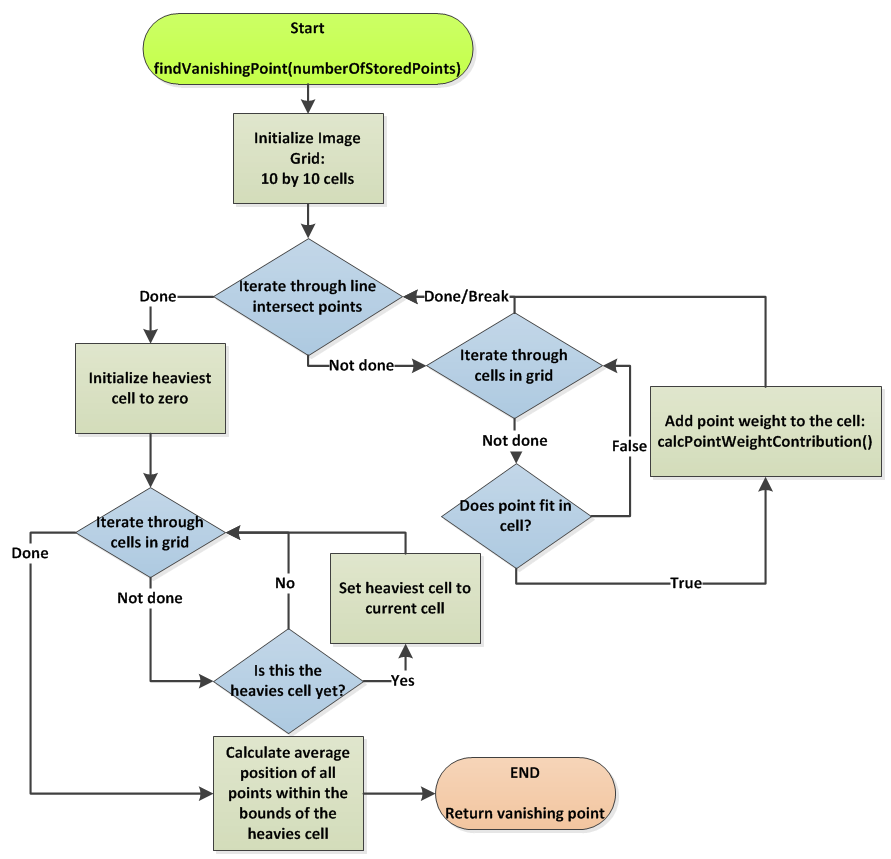
\includegraphics[scale=0.5]{findVp}
	\caption{Sequence diagram illustrating program execution when the user activates camera feed and VP detection.}
	\label{fig:findVp}
\end{figure}

\subsection{Vanishing Point Detector Application}

\paragraph{Program Structure}

The vanishing point detector was implemented as a QWidget Application in the Qt Creator IDE. The code excerpt shown in algorithm \ref{alg:edgelines} contains the most important image processing steps. A main thread, which may be called the GUI thread, handles all user related input and output. All image processing is done in the class \textit{ImageProcessing} which inherits from QThread. This means that \textit{ImageProcessing} controls a protected function \textit{run()} which contains the threaded code and image processing steps. Figure \ref{fig:VpAppSequence} is a sequence diagram that shows the different classes and threads interact. The ellipse filter step is ommitted in the illustration; if it had been included, it would be called between \textit{hough->detect()} and \textit{getVanishingPoint()}.

\begin{algorithm}[h]
	\caption{Vanishing point detector loop. Several lines of code are omitted in this example to make the processing more clear.}
	\label{alg:edgelines}
	\begin{verbatim}
	while(){
	    capture.read(cameraImg);
	    cvtColor(cameraImg,grayImg,CV_RGB2GRAY);
	    blur( grayImg, blurredImg, Size(3,3) );
	    Canny(blurredImg, edgesImg, lowerThresh, upperThresh, 3);
	    gpu_edgesImg.upload(edgesImg);
	    lines = detectHoughLines(gpu_edgesImg);   
	    newLines = mLineEllipseFilter.filterLines(lines,originalImage);
	    Point vanishingPoint = vpDetector.getVp(newLines,cameraImg);     
	}
	\end{verbatim}
\end{algorithm}

\begin{landscape}
	\begin{figure}
		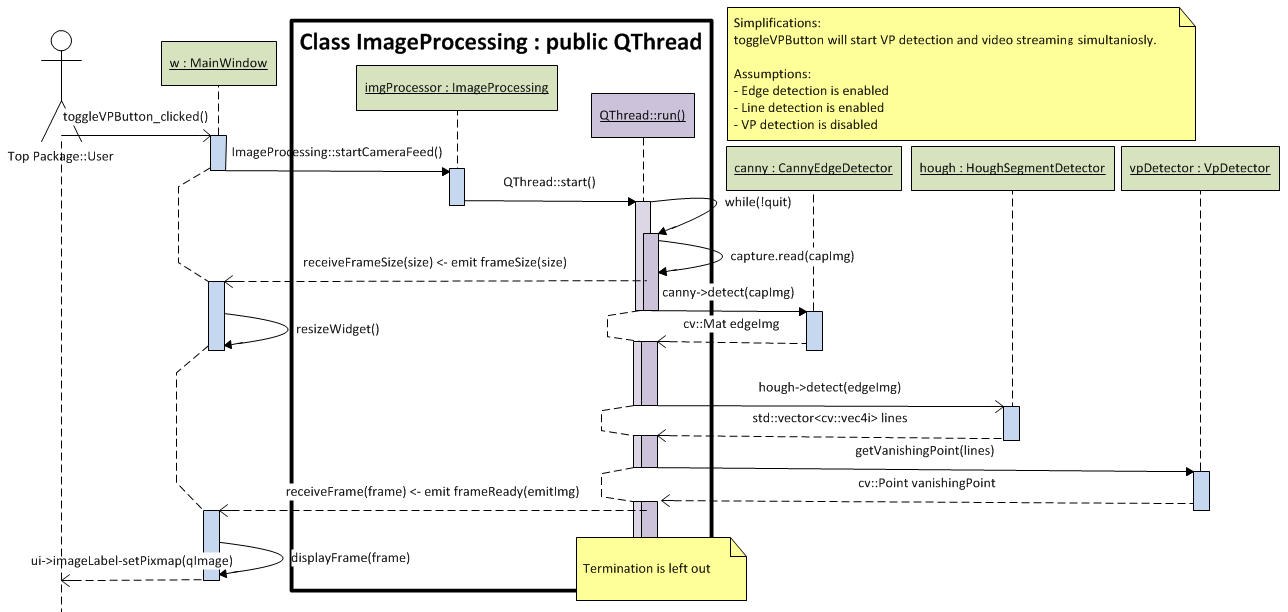
\includegraphics[scale=0.55]{VpAppSequence}
		\caption{Sequence diagram illustrating program execution when the user activates camera feed and VP detection.}
		\label{fig:VpAppSequence}
	\end{figure}
\end{landscape}



\paragraph{Graphical User Interface}

A graphical user interface was created so that the parameters for the canny edge detector and Hough lines detector could be tuned on-line. All widgets shown in figure \ref{fig:vpGui} have their functionality implemented. The user can turn on the camera feed, in this case from the web camera integrated into the laptop of the author, and switch line and edge detection on or off. Upper and lower edge detection thresholds, as well as line detection parameters can be set by using the sliders. The kernel size for the edge detector is set to 3 by 3, and can not be changed by the user. When both edge detection and line detection is enabled, the user may turn on the vanishing point detector module. In this particular application, the ellipse line filter module is not included.

\begin{figure}
	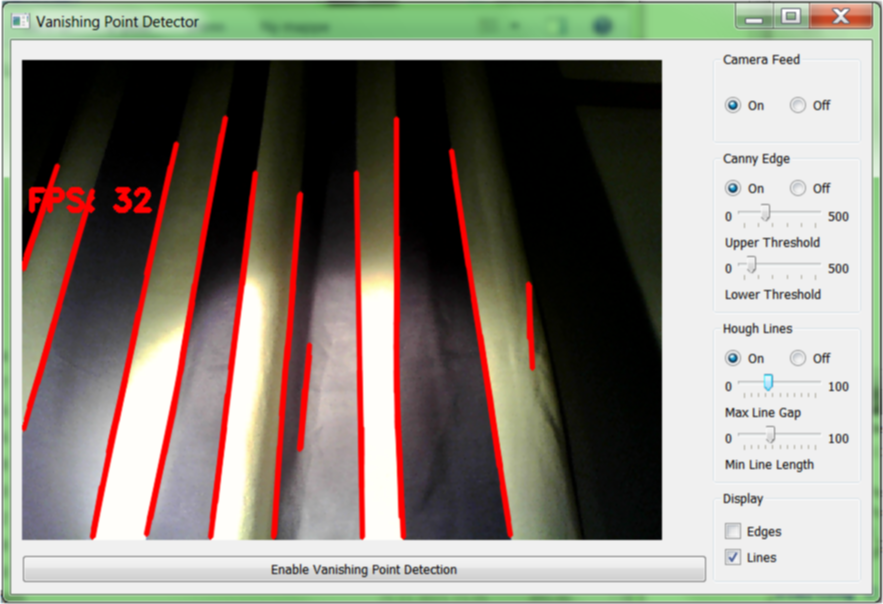
\includegraphics[scale=0.7]{VPGuiBlurred}
	\caption{Graphical user interface for the vanishing point detector. Note that the detected line segments are actually several lines overlapping each other.}
	\label{fig:vpGui}
\end{figure}

\subsection{Cause of Failure}

\section{Depth Perception and Obstruction Detection}

\subsection{Overview}

\subsection{The camera rig}

The two IP cameras were moved together to form a stereo camera. This stereo camera was used in two positions. The first camera position is on the pan-tilt module on the robot arm, see figure \ref{fig:rig_pantilt}. The second position is just over the LIDAR in front of the robot arm base, see figure \ref{fig:rig_front}.  The workshop at \gls{itk} made a mounting bracket, so that the cameras could be placed over the LIDAR. In stereo vision, it is essential that the positions of the cameras relative to each other is constant. One problem encountered throughout the project was that the camera assemby, when placed either at the pan-tilt module and over the LIDAR, was not rigid enough. The severity of this problem was somewhat alleviated by wrapping a strap around both the cameras. This camera rig is ad hoc, i.e. suitable for the purpose of this project, and a better solution should be used for succeeding projects.

\begin{figure}
	\centering
	\begin{subfigure}[b]{0.45\textwidth}
		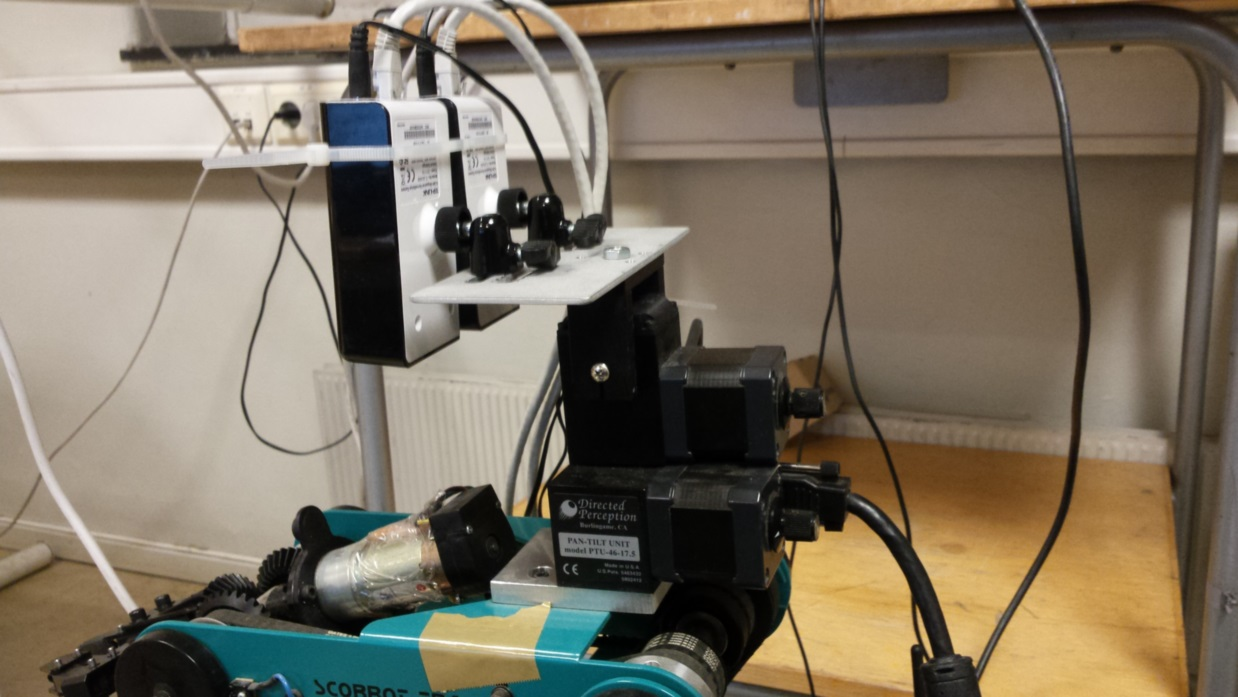
\includegraphics[width=\textwidth]{rig_pantilt}
		\caption{Camera pair mounted on the pan-tilt module.}
		\label{fig:rig_pantilt}
	\end{subfigure}
	\begin{subfigure}[b]{0.45\textwidth}
		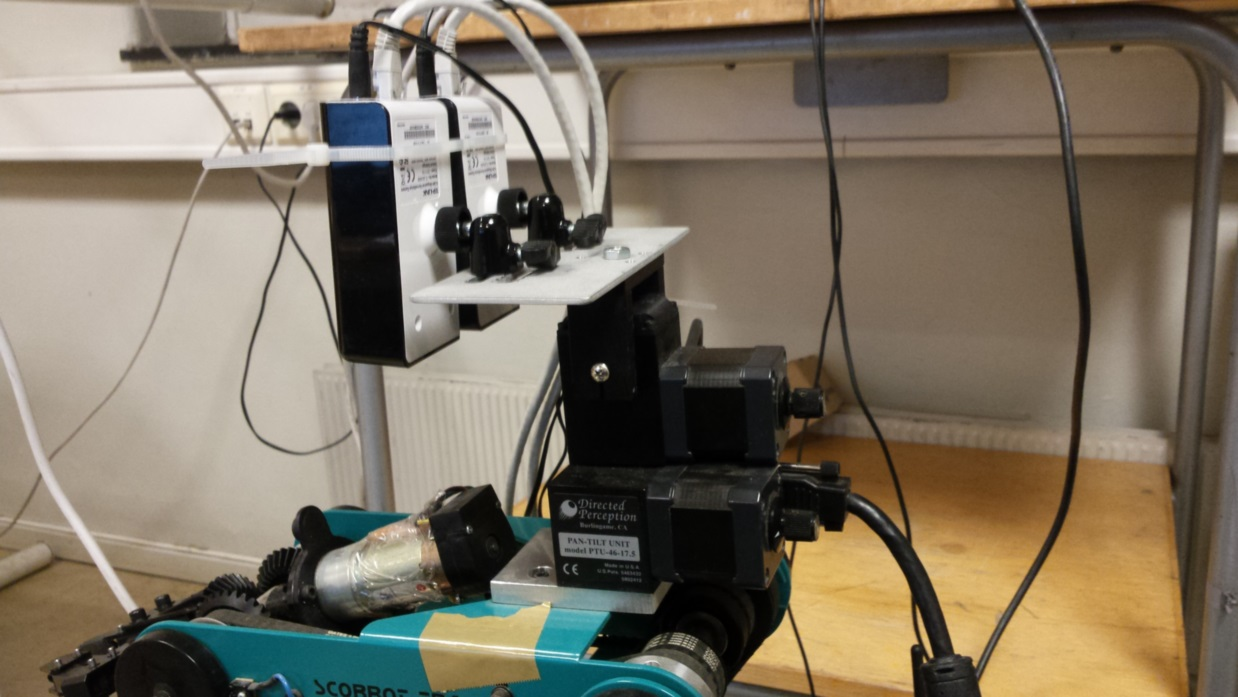
\includegraphics[width=\textwidth]{rig_pantilt}
		\caption{Camera pair mounted on the pan-tilt module.}
		\label{fig:rig_front}
	\end{subfigure}
	\caption{\label{fig:campos}The two camera positions.}
\end{figure}

\subsection{Graphical User Interface}

Tuning the parameters for stereo matching in OpenCV is a wearisome task, especially without a good graphical user interface. Figure \ref{fig:StereoGui} shows the user interface which was used to observe how parameter tuning alters the disparity map quality. Not all functionalities were implemented.

\begin{figure}
	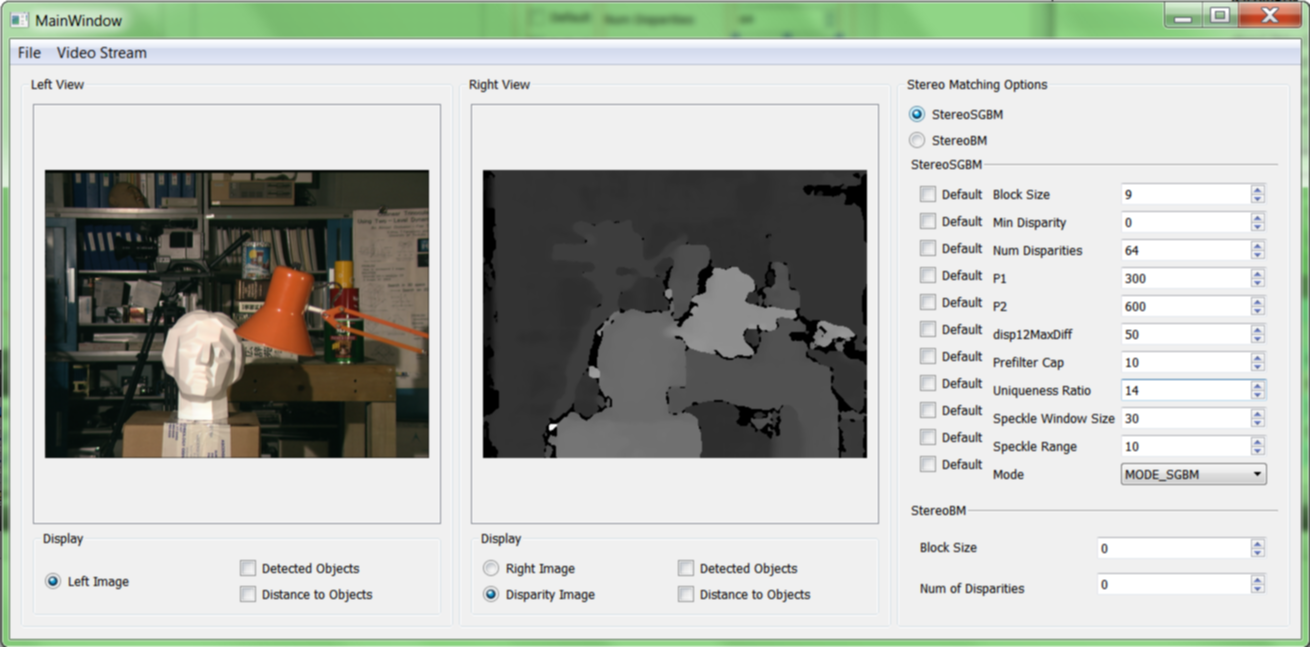
\includegraphics[scale=0.37]{StereoGui}
	\caption{Graphical user interface for stereo matching. A disparity map is computed from the Tsukuba samples by using StereoSGBM. }
	\label{fig:StereoGui}
\end{figure}

\subsection{Calibration}

As mentioned in chapter \ref{chp:theory}, all cameras will have some distortion. If the distortion is too severe, as it often will be in the context of stereo vision, the camera must be calibrated. In addition, it was assumed that the image planes were located on the same plane, and that a projection pair, for example the projections $X_L$ and $X_R$ of an object $X$, form two equal epipolar lines, $e_1$ and $e_2$, on the two image planes. In practice, these conditions are achieved through stereo calibration. The second purpose of the calibration procedure is to relate the sensor data to real world quantities, in order to measure the distance to detected objects. Code listings from Practical OpenCV by Samarth Brahmbhatt \cite{practicalopencv} has been used as a basis for calibration in this project. Some parts of his code is almost unchanged, while other parts of the listings are altered and expanded significantly. There are three steps in the calibration procedure:

\begin{enumerate}
	\item Single camera calibration: 
	\item Stereo calibration.
	\item Image rectification.
\end{enumerate}

See figure \ref{fig:calibproc} for an overview of the calibration procedure. All these steps require a familiar object with known dimensions to calibrate against. Among the three calibration patterns supported by OpenCV, this implementation utilized a black and white chessboard. The chessboard has 6 by 8 squares with sides $\approx 26 \, mm$ long.

\begin{figure}
	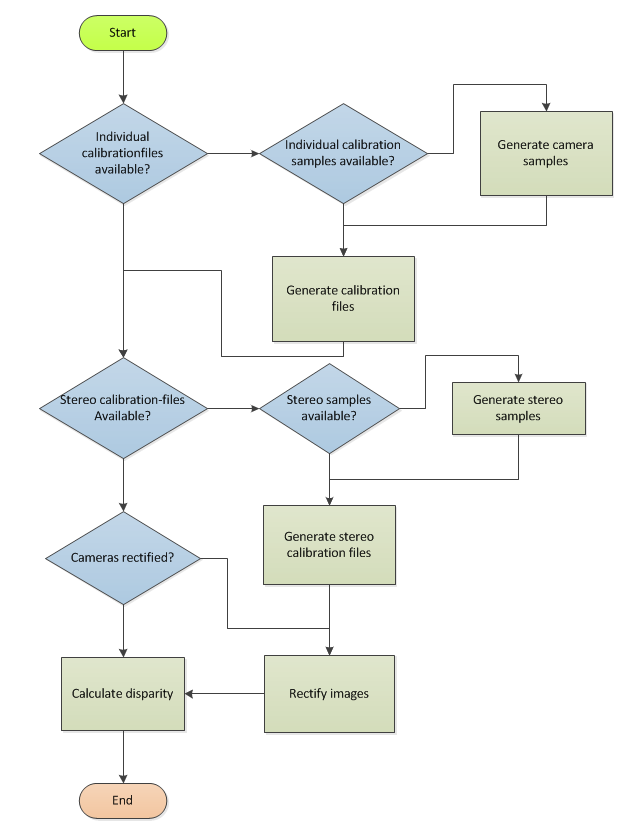
\includegraphics[scale=0.7]{StereoInit}
	\caption{An overview of the calibration procedure.}
	\label{fig:calibproc}
\end{figure}

\begin{figure}
	\centering
	\begin{subfigure}[b]{0.90\textwidth}
		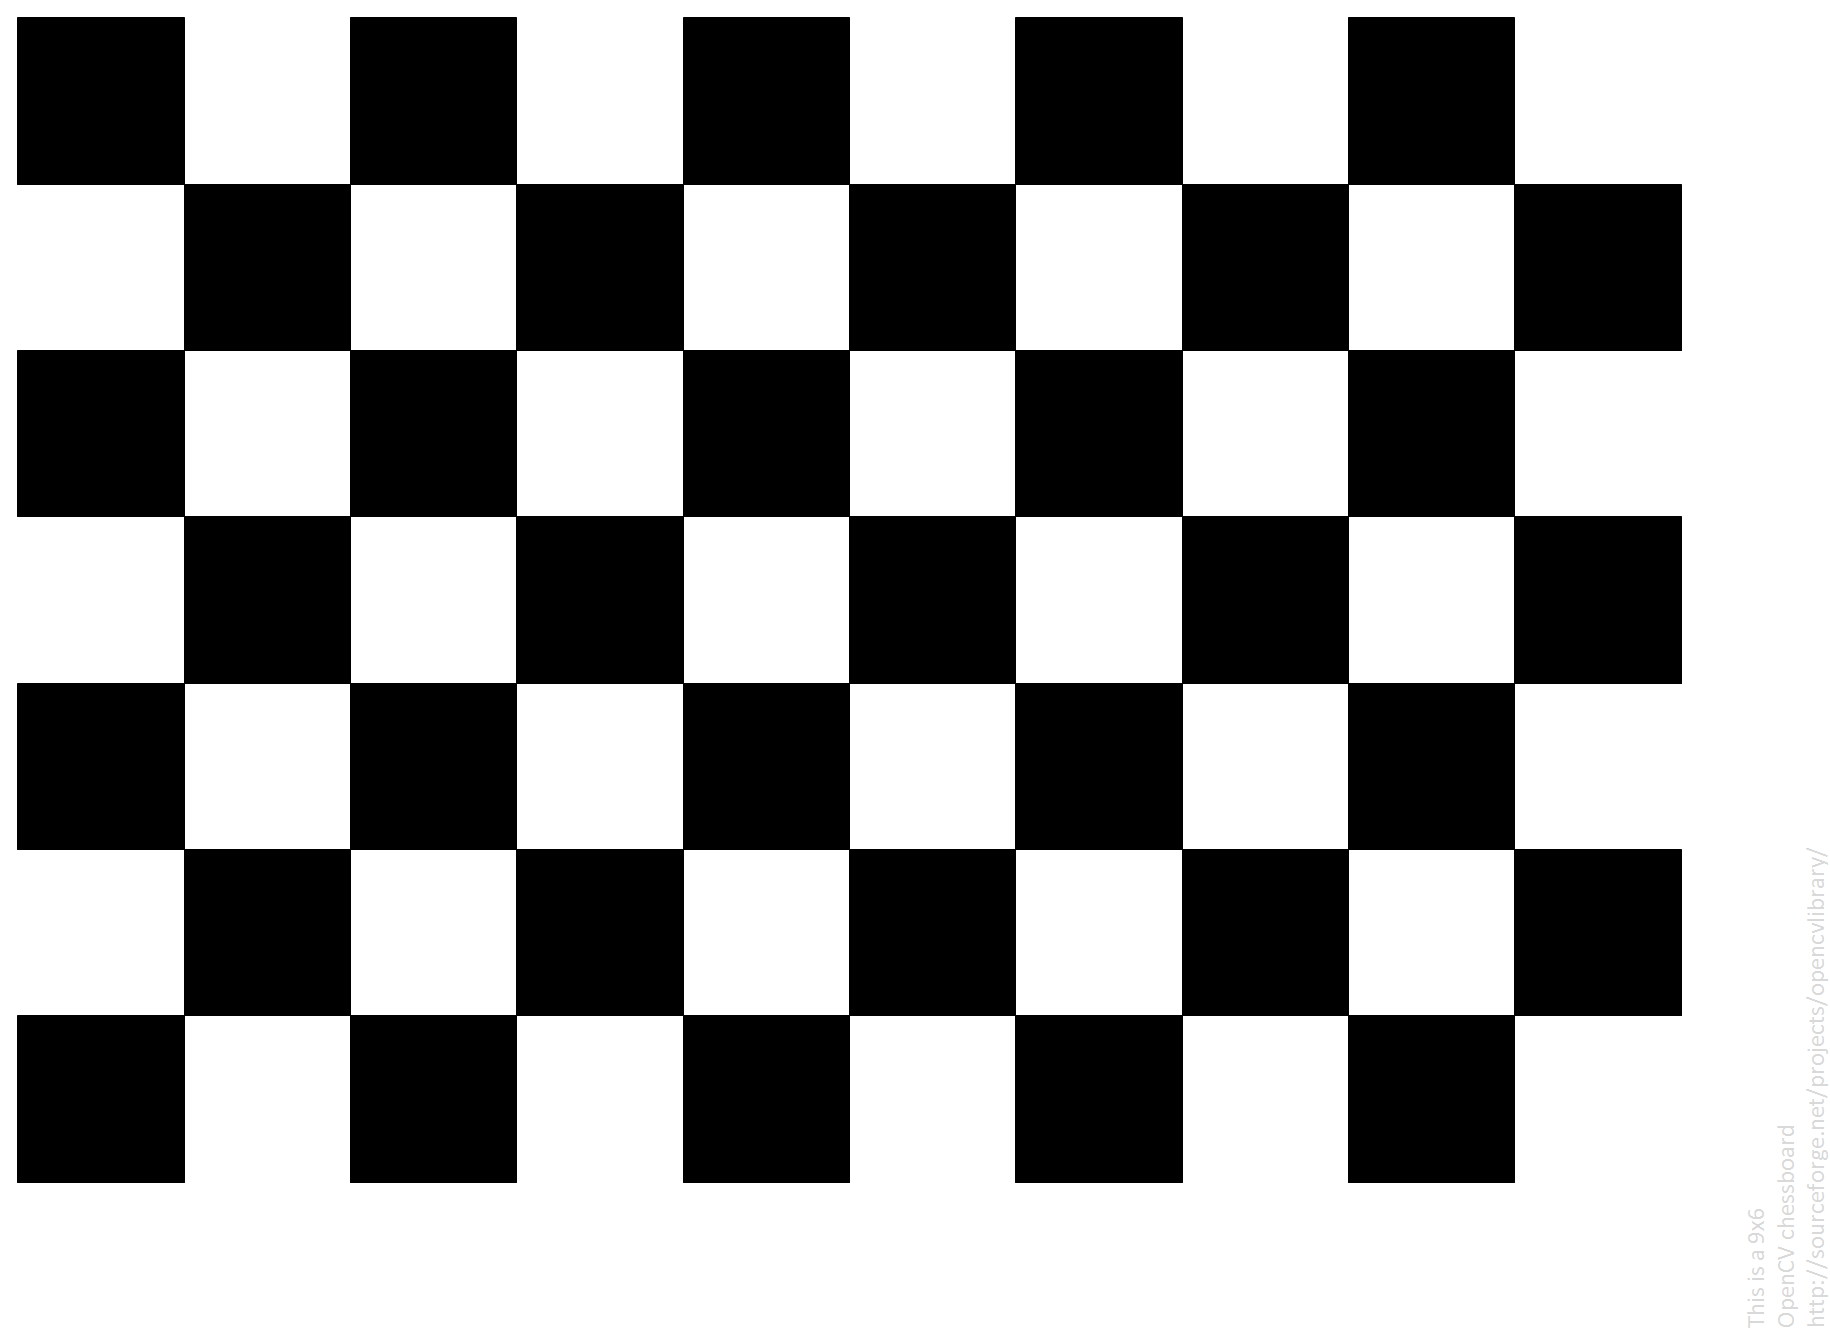
\includegraphics[width=\textwidth]{chess_pattern}
		\caption{The chessboard calibration pattern. The pattern was printed and taped to a flat surface.}
		\label{fig:chesspattern}
	\end{subfigure}
	\begin{subfigure}[b]{0.90\textwidth}
		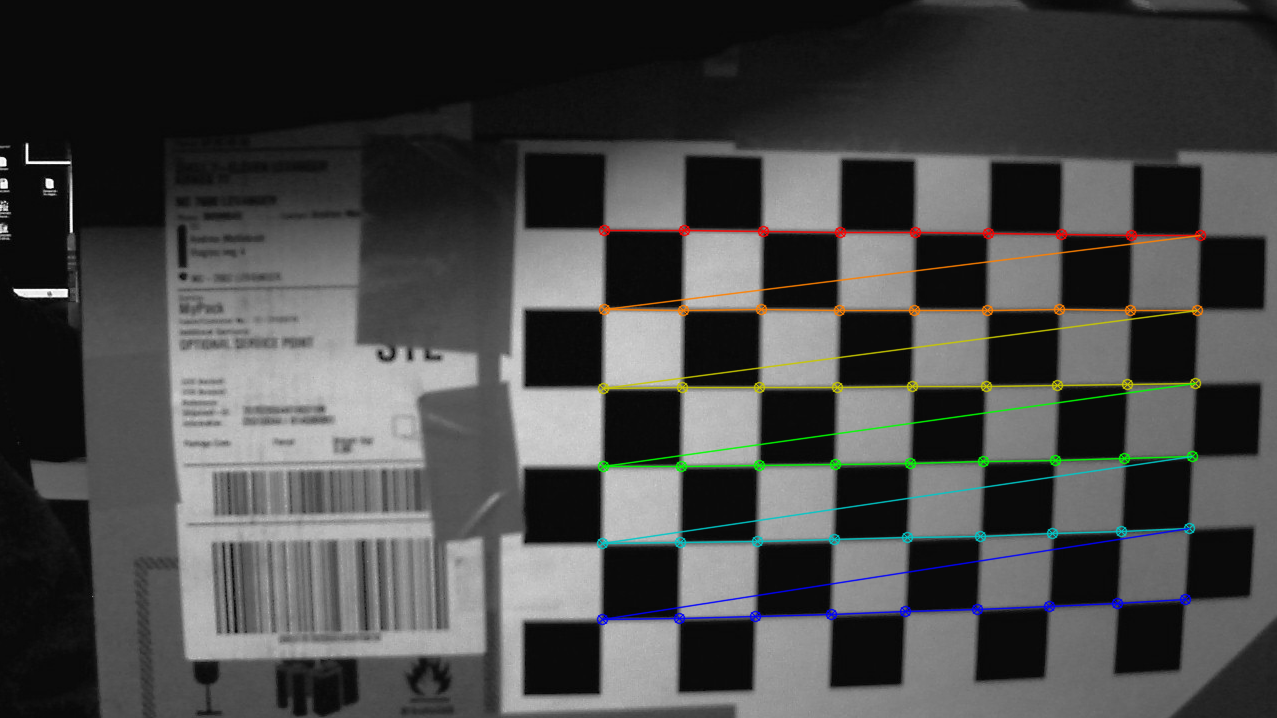
\includegraphics[width=\textwidth]{CamCalibDistorted}
		\caption{Chessboard detection. This is one of the sample images used to calibrate the camera. Notice the distortion in the lower right corner.}
		\label{fig:chessdetection}
	\end{subfigure}
	\caption{\label{fig:calibrationpattern}}
\end{figure}

\paragraph{Single Camera Calibration}

\begin{wrapfigure}{r}{0.48\textwidth}
	\vspace{-10pt} % Remove exessive whitespace
	\centering
	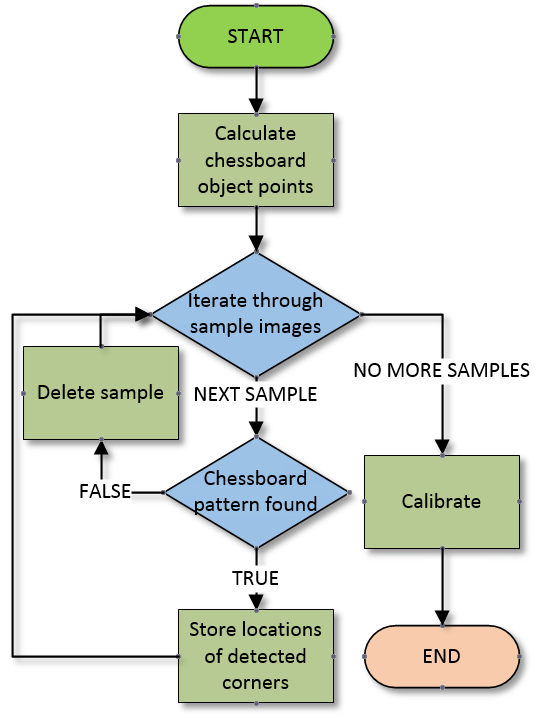
\includegraphics[width=0.50\textwidth]{singleCamCalib}
	\caption{\label{fig:singleCamCalib} Single camera calibration.}
	\vspace{-20pt} % Remove exessive whitespace
\end{wrapfigure}

In this step, the cameras are calibrated separately.  The purpose of this calibration procedure is to counter the constant radial and tangential distortion in a pinhole camera, and to identify the pinole camera model. The result of this procedure is the 3 by 3 camera matrix and the five distortion coefficients mentioned in the theory chapter. In the flowchart in figure \ref{fig:singleCamCalib}, assume that enough useful sample images are gathered and read into the program. In the last step, \gls{opencv}s calibration function will take inn the detected corners from the sample images and the chessboard dimentions. Finally, the calibration results are stored in an .xml file:

\begin{verbatim}
<?xml version="1.0"?>
<opencv_storage>
<cameraMatrix type_id="opencv-matrix">
  <rows>3</rows>
  <cols>3</cols>
  <dt>d</dt>
  <data>
    1.4478141049219482e+003 0. 6.6274484776761142e+002 
    0. 1.4432743079138295e+003 4.7609546427843065e+002 
    0. 0. 1.
  </data></cameraMatrix>
<distCoeffs type_id="opencv-matrix">
  <rows>1</rows>
  <cols>5</cols>
  <dt>d</dt>
  <data>
    -2.6128696949919589e-001 3.4600669963821584e-001
    -2.2331413545278616e-003 -2.5710895791919218e-003
    -3.7144316064113458e-001</data></distCoeffs>
</opencv_storage>
\end{verbatim}

\newpage



When all the image samples has been read into the program, the program will check if the chessboard can be detected. If the chessboard is present in the image, the position of the corners will be stored in  

\paragraph{Stereo Calibration}

Stereo calibration is almost exactly the same as single camera calibration. An important difference is obviously that sample images must be taken from both cameras simultaniously. The calibration pattern must be detectable in both frames. Stereo calibration will generate a new set of data:

\begin{description}
	\item[R: ] 3 by 3 rotation matrix between the two cameras.
	\item[T: ] Translation between the two cameras. Denoted $B$ in the theory chapter. Relates the left camera to the right together with $R$. 
	\item[E: ] 3 by 3 essential matrix.
	\item[F: ] 3 by 3 fundamental matrix.
\end{description}

These matrices will be stored in a new file, ''stereo\_calib.xml'', together with the distortion coefficients and camera matrices from the two single camera calibrations. These values will be applied in the next calibration step.

\paragraph{Stereo Rectification}

Rectification is the final step before stereo matching can be performed. In this step, the information that is necessary to align the stereo frames. When the frames are aligned, Rectification is completed by:

\begin{enumerate}
	\item Loading ''stereo\_calib.xml'' and reading in the camera matrices, distortion coefficients, $R$ and $T$.
	\item Calling \textit{stereoRectify()} with the data above as input.
\end{enumerate}

 \textit{stereoRectify()} will write data onto a set of new matrices:

\begin{description}
	\item[Rl: ] 3 by 3 rotation matrix for the left frame.
	\item[Rr: ] 3 by 3 rotation matrix for the right frame.
	\item[Pl: ] 3 by 4 left projection matrix.
	\item[Pr: ] 3 by 4 right projection matrix.
	\item[Q: ] 4 by 4 reprojection matrix. Maps disparity to depth.

\end{description}

Finally, the function \textit{initUndistortRectifyMap()} will use these matrices to generate four pixel maps with a size that equals the input images. The pixel maps are added the ''stereo\_calib.xml''. These matrices maps the pixels in the original images to their rectified locations. To rectify an input image, call the function \textit{remap()}.

\begin{verbatim}
	remap(leftCameraFeed, leftCameraFeed_rect, map_l1, map_l2, INTER_LINEAR);
\end{verbatim}

In this example, the function takes in the left camera feed and the \textit{cv::Mat} that will hold the resulting rectified image. \textit{map\_l1} and \textit{map\_l2} are the pixel maps. The result of all the calibration steps and the final rectification step is shown in figure \ref{fig:calibBeforeAfter}.

\begin{figure}
	\centering
	\begin{subfigure}[b]{0.95\textwidth}
		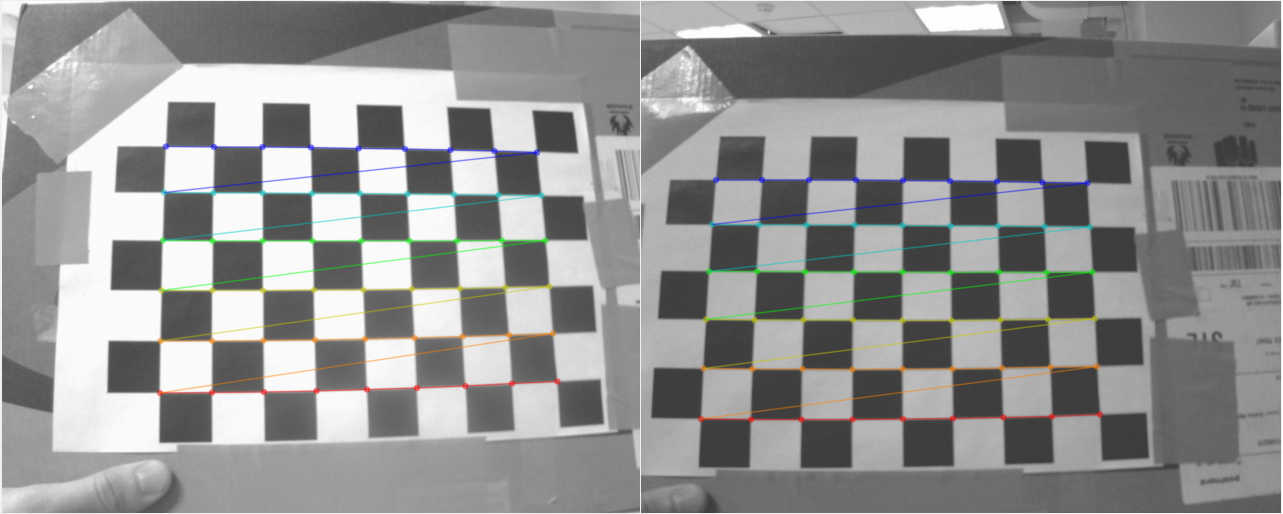
\includegraphics[width=\textwidth]{stereoPreCal}
		\caption{Before calibration and rectification.}
		\label{fig:stereoPreCal}
	\end{subfigure}
	\begin{subfigure}[b]{0.95\textwidth}
		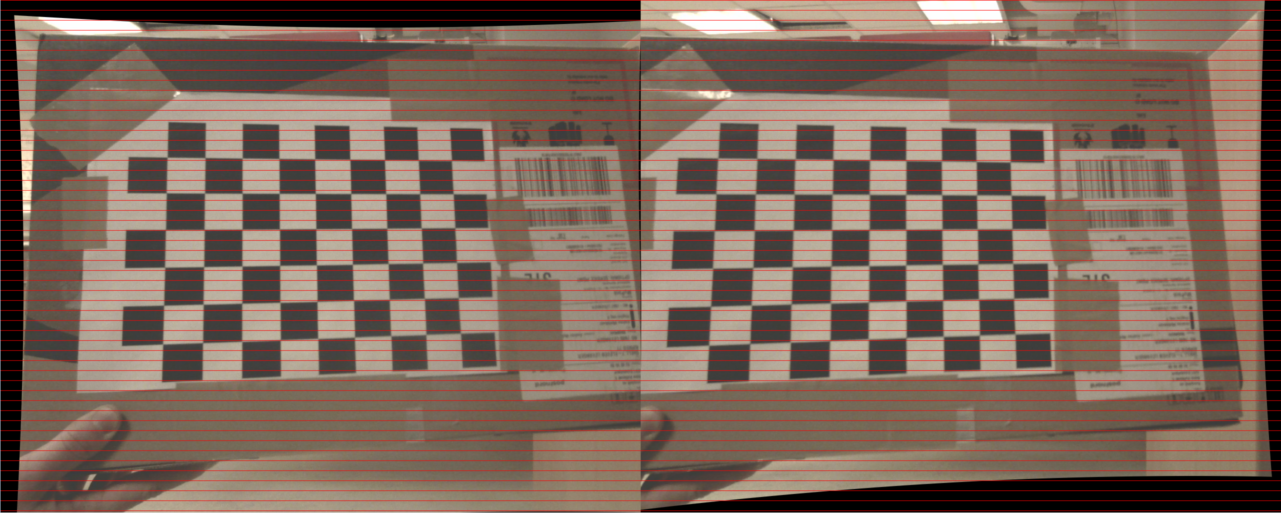
\includegraphics[width=\textwidth]{stereoPostCal}
		\caption{After calibration and rectifivation.}
		\label{fig:stereoPostCal}
	\end{subfigure}
	\caption{\label{fig:calibBeforeAfter}Before and after calibration. The red lines in \ref{fig:stereoPostCal} can be used to assess the quality of the calibration procedure. Note that these image pairs are captured at different times.}
\end{figure}

%\begin{figure}
%\includegraphics[scale=•]{•}
%\end{figure}

\subsection{Stereo Matching}

Recall that stereo matching is the search for mutual information in the sereo image pair. Matching of the sterao pair will result in a single channel disparity image (figure \ref{fig:StereoMatching}), i.e. the pixels have intencity values along a single dimention. The disparity is a measure of how far a block of features has shifted between the left and right image. 

\begin{figure}
	\centering
	\begin{subfigure}[b]{0.45\textwidth}
		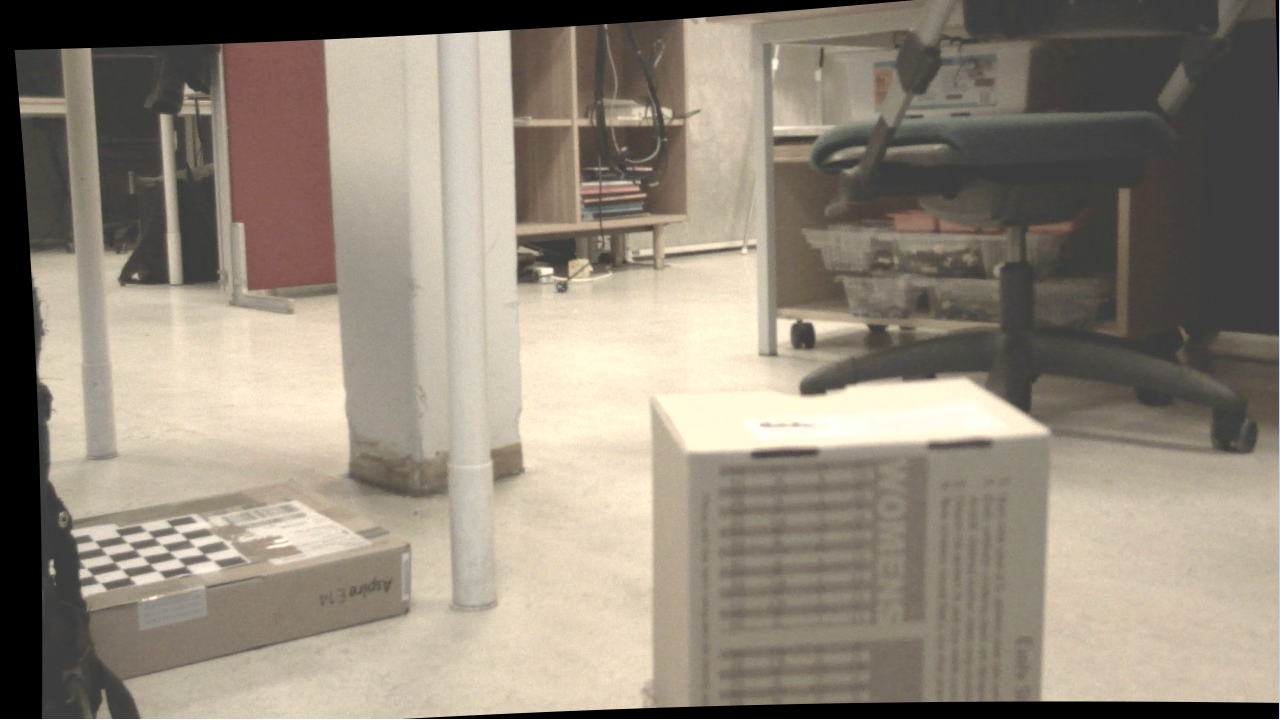
\includegraphics[width=\textwidth]{OriginalExample}
		\caption{Left camera image.}
		\label{fig:OriginalExample}
	\end{subfigure}
	\begin{subfigure}[b]{0.45\textwidth}
		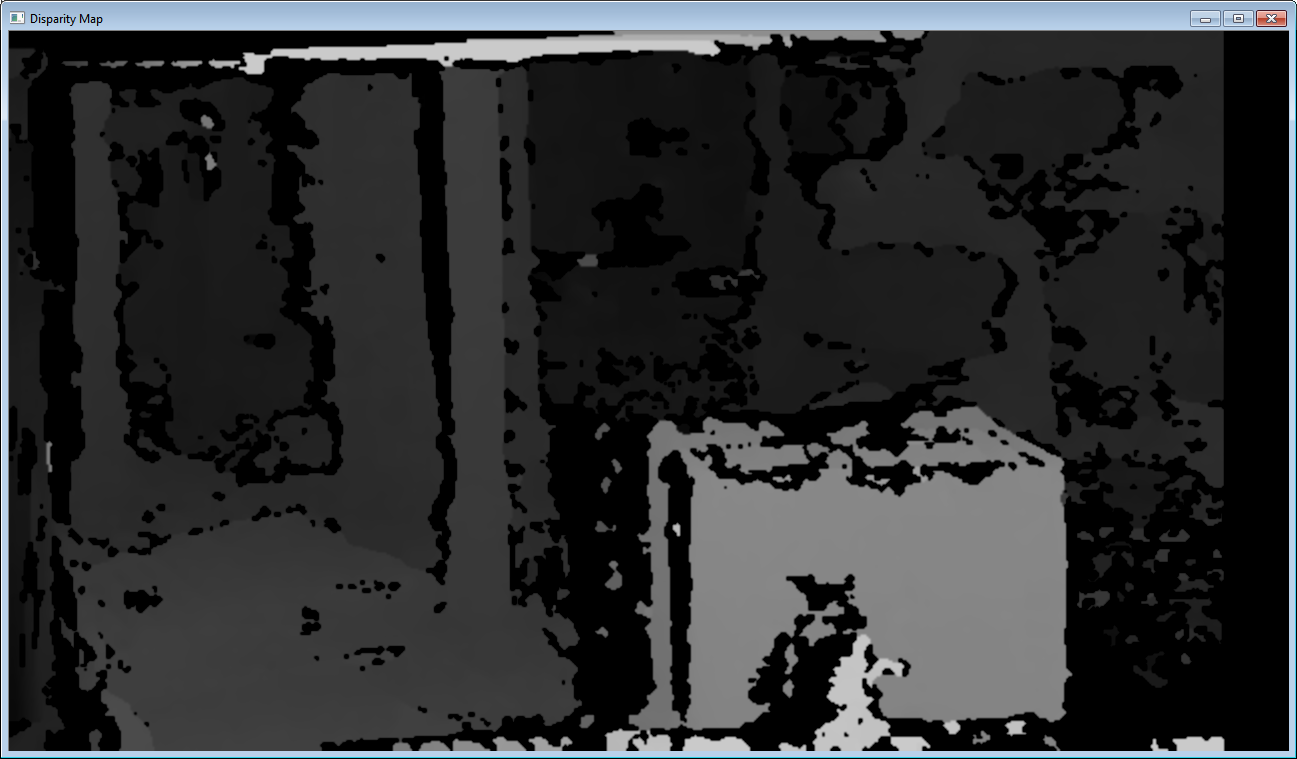
\includegraphics[width=\textwidth]{DispExample}
		\caption{Disparity map.}
		\label{fig:DispExample}
	\end{subfigure}
	\caption{\label{fig:StereoMatching}The result of StereoSGBM.}
\end{figure}

\paragraph{Processing Time}
In this application, with no hardware acceleration from CUDA and the like, the choice of matching algorithm stands between the regular StereoBM and the more robust StereoSGBM. Block Matching (BM) is the fastest of the two, and usually allows a frame rate of several frames per second. Semi Global Block Matching (SGBM) on the other hand, is much slower. The Tsukuba samples in figure \ref{fig:StereoGui} are 384 pixels wide by 288 pixels high. Matching them with StereoSGBM takes roughly half a second. Images from the IP cameras on the robot are set to be 1280 pixels wide by 1024 pixels high. In this case, matching with StereoSGBM takes approximatly 8 seconds; a processing time which is too long if it is to be used for navigation. A solution to this problem is to reduce the size of the image pair. This was done in the matching application by downsampling the input images to $1/4th$ of their original size by using \textit{pyrDown()} in \gls{opencv}. This brings the frame rate up to 2 frames per second.

The StereoSGBM object require at least these parameters:

 \begin{description}
 	\item[numDisparities: ] The number of disparity values, and indirectly the maximum left to right projection displacement. Must be divisible by 16.
 	\item[minDisparity: ] The lowest disparity to be computed.
	\item[blockSize: ] A block of pixels. Defines the size of regions to be matched. Must be an odd number, because the block is centered around a pixel.
\end{description}

Selecting a block size is a compromize between robustness and level of detail. Consider a block with the size of a single pixel. It is highly probable that it will cause false matches. A too large block will generate less noisy matches, while the details are surpressed.

\begin{figure}
	\centering
	\begin{subfigure}[b]{0.30\textwidth}
		\includegraphics[width=\textwidth]{blockSize1}
		\caption{Block size $= 1$.}
		\label{fig:block1}
	\end{subfigure}
	\begin{subfigure}[b]{0.30\textwidth}
		\includegraphics[width=\textwidth]{blockSize9}
		\caption{Block size $= 9$.}
		\label{fig:block9}
	\end{subfigure}
	\begin{subfigure}[b]{0.30\textwidth}
		\includegraphics[width=\textwidth]{blockSize25}
		\caption{Block size $= 25$.}
		\label{fig:block21}
	\end{subfigure}
	\caption{\label{fig:blockSize}Comparison of different block sizes.}
\end{figure}


\subsection{Finding Obstructions}

\begin{figure}
	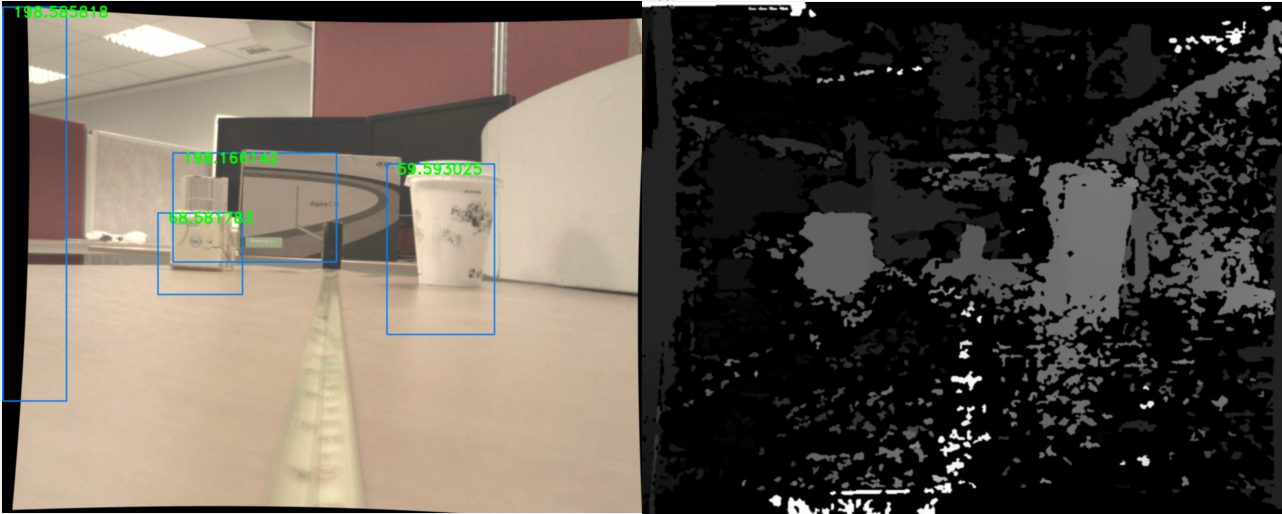
\includegraphics[scale=0.37]{obstruction}
	\caption{A preliminary version of the obstruction detector}
	\label{fig:obstruction}
\end{figure}

Detection of obstructions is based purely on color thresholding, and is performed in the custom made: \textit{DepthFilter} class. The idea and initial code for obstruction detection is based on this autor's very first meeting with \gls{opencv}: an object tracking tutorial by \href{https://www.youtube.com/watch?v=bSeFrPrqZ2A}{Kyle Hounslow on youtube.com}. In the implemented application, obstruction detection is done within the \textit{DepthFilter} class. After the disparity map is calculated, the disparity thread will call \textit{exctractObstructions()} within the \textit{DepthFilter} class. The program flow within the function is shown in figure \ref{fig:obstructionFlow}. All detected obstructions are indicated on the original left frame by bounding rectangles (figure \ref{fig:obstruction}). The most sentral parts of the flowchart inf figure \ref{fig:obstructionFlow} will be explained in detail.

\begin{figure}
	\centering
	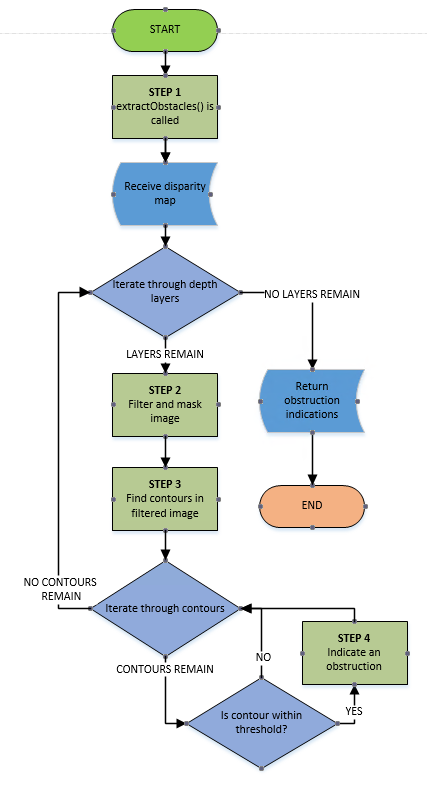
\includegraphics[width=0.8\textwidth]{obstructionFlow}
	\caption{Obstruction detection in \textit{DepthFilter}.}
	\label{fig:obstructionFlow}
\end{figure}

\begin{wrapfigure}{l}{0.4\textwidth}
	\centering
	
	\begin{subfigure}[b]{0.35\textwidth}
		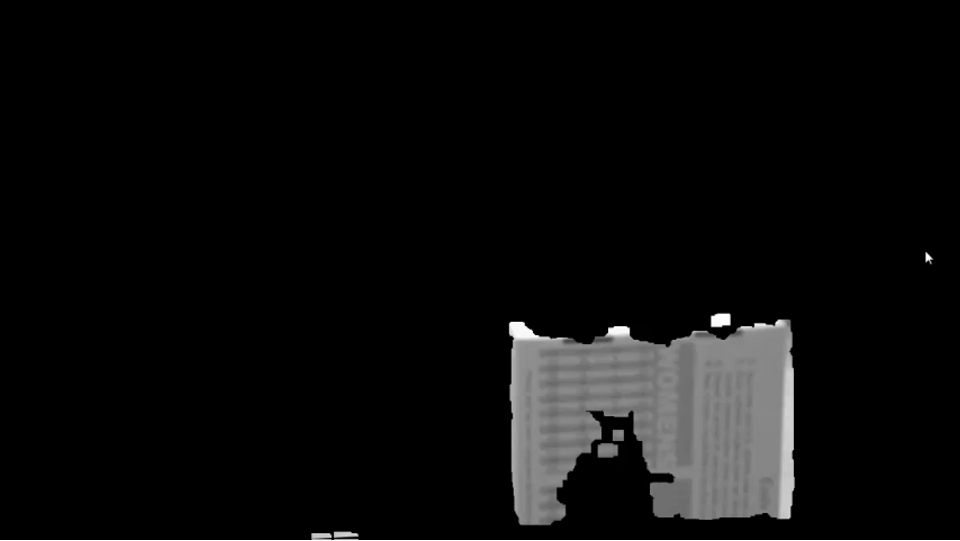
\includegraphics[width=\textwidth]{DepthLayer1}
	\end{subfigure}
	\par\medskip
	\begin{subfigure}[b]{0.35\textwidth}
		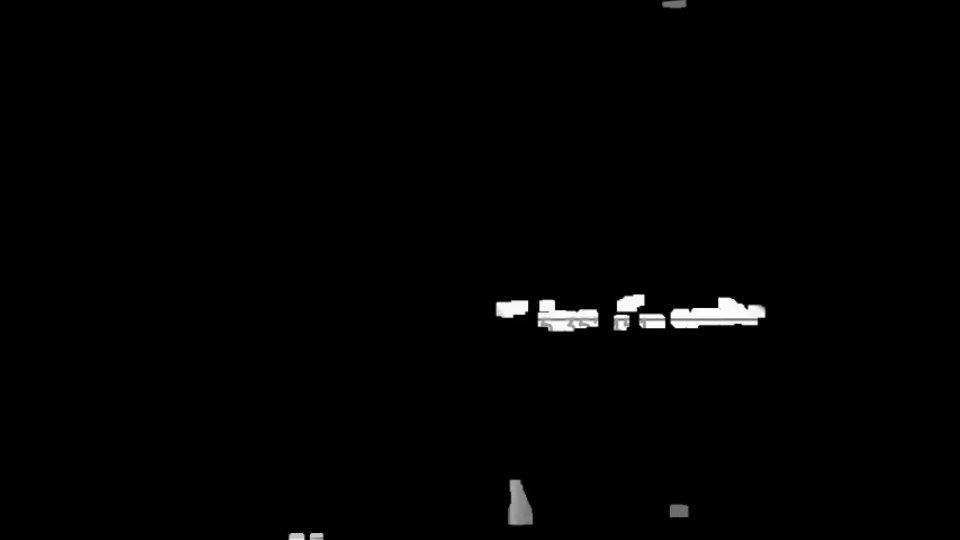
\includegraphics[width=\textwidth]{DepthLayer2}
	\end{subfigure}
	\par\medskip
	\begin{subfigure}[b]{0.35\textwidth}
		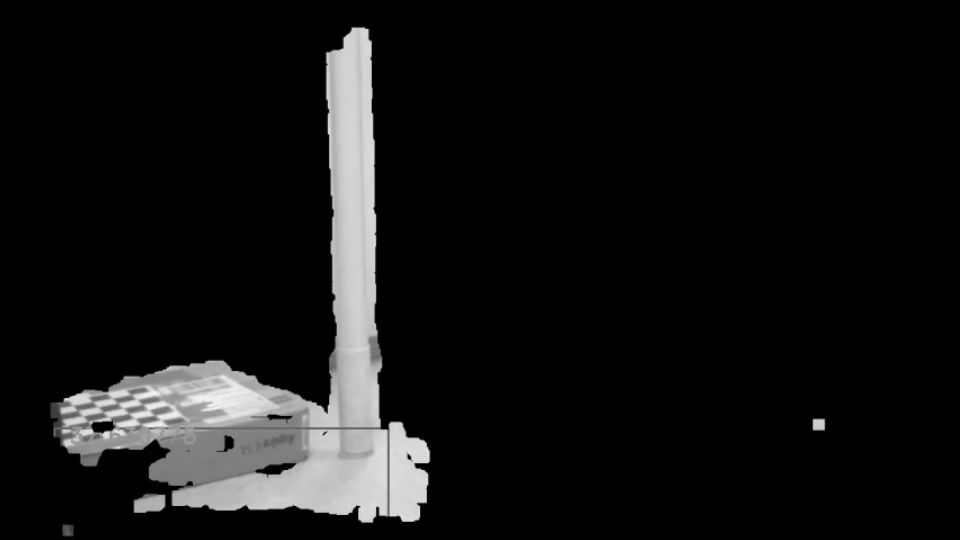
\includegraphics[width=\textwidth]{DepthLayer6}
	\end{subfigure}
	\par\medskip
	\begin{subfigure}[b]{0.35\textwidth}
		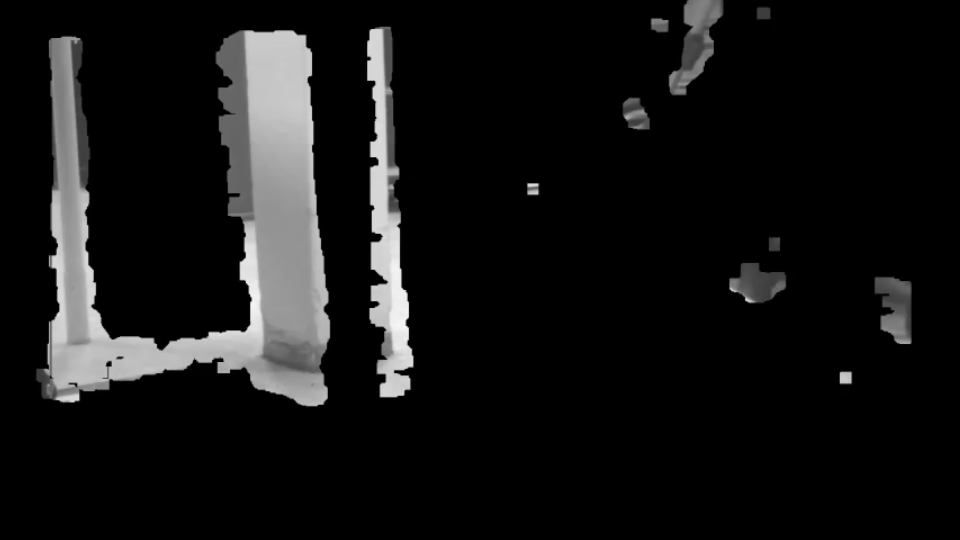
\includegraphics[width=\textwidth]{DepthLayer7}
	\end{subfigure}
	\par\medskip
	\begin{subfigure}[b]{0.35\textwidth}
		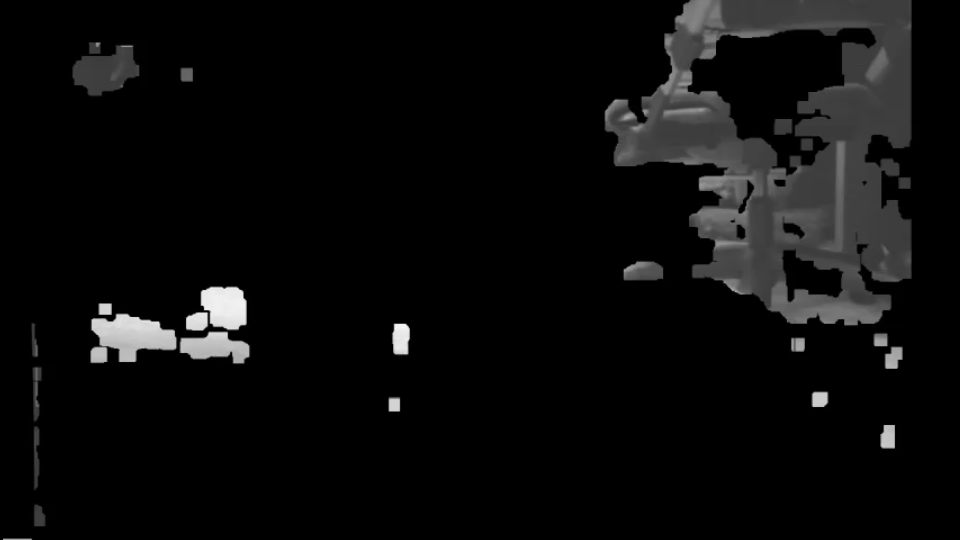
\includegraphics[width=\textwidth]{DepthLayer8}
	\end{subfigure}
	
	\caption{Some of the depth layers in figure \ref{fig:StereoMatching} separated by color filtering. The top image is the closest layer, while the most distant layer is at the bottom.}
	\label{fig:layers2}
\end{wrapfigure}

\paragraph{Iterate Through Depth Layers}

Disparity range is set to $\{0 ... 160 \}$, where each value relates to a corresponding distance. This part of the code will iterate through disparity intervals with a constant size of 10 starting at an interval of $\{150 ... 160\}$, and ending at $\{20 ... 30 \}$. The idea behind these intervals is that possible obstructions will stand out from the surface of the ground level (floor) and form a distinct shape that can be separated from the surroundings.

\paragraph{Filter and Mask Image}

This step will produce a binary image which represents the region of the disparity image where the disparity values falls within the interval from the previous step. This binary image is filtered by eroding all features with a size smaller than a predetermined value.

\paragraph{Find Contours}

It is possible to detect a set of contours in the filtered binary image. This is done with a prebuilt function from the OpenCV library.

\paragraph{Iterate Through Contours and Indicate Obsticles}

Some of the contours are so small that they can either be considered to be noise or harmless obsticles. Contours with an area above a certain size are also rejected. Rejecting large contours may seem to be a bad decision, but is is necessary given the limitations of this implementaton\ref{chp:assessment}. The contours are then indicated by a bounding rectangle.

\subsection{Distance Measurment}

Another functionality implemented within the \textit{DepthFilter} class is the ability to calculate the distance from the camera to the detected contours. 

\begin{figure}
	\centering
	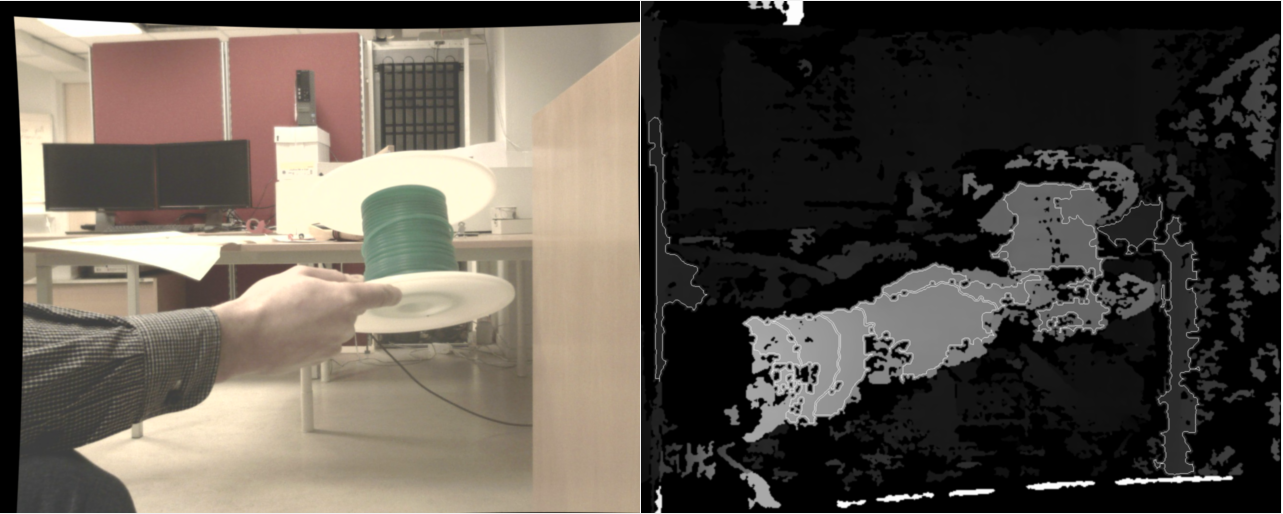
\includegraphics[width=1\textwidth]{contourDetection}
	\caption{All the detected contours in a disparity map that falls within the size threshold.}
	\label{fig:contourDetection}
\end{figure}

\begin{wrapfigure}{r}{0.48\textwidth}
	\vspace{-10pt} % Remove exessive whitespace
	\centering
	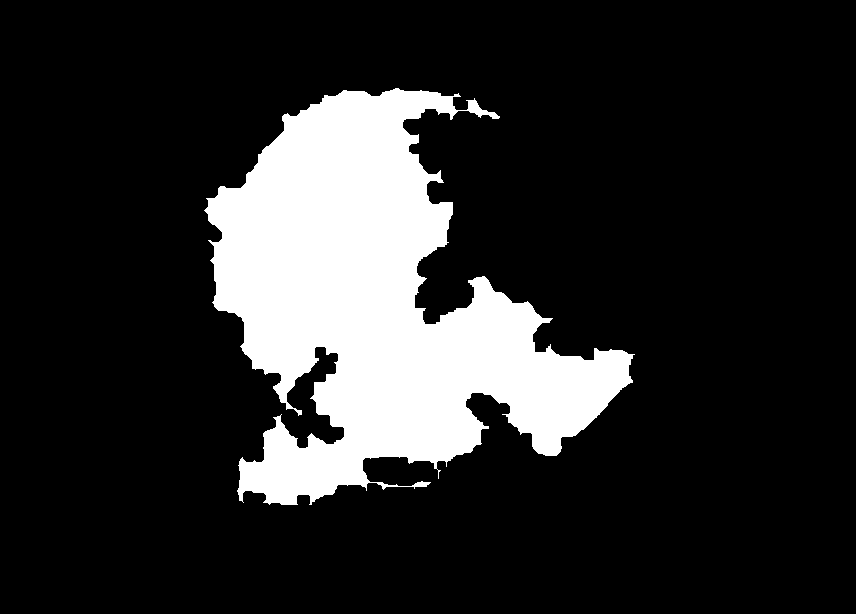
\includegraphics[width=0.50\textwidth]{mask}
	\caption{\label{fig:mask} A mask.}
	\vspace{-20pt} % Remove exessive whitespace
\end{wrapfigure}

\begin{figure}
	\centering
	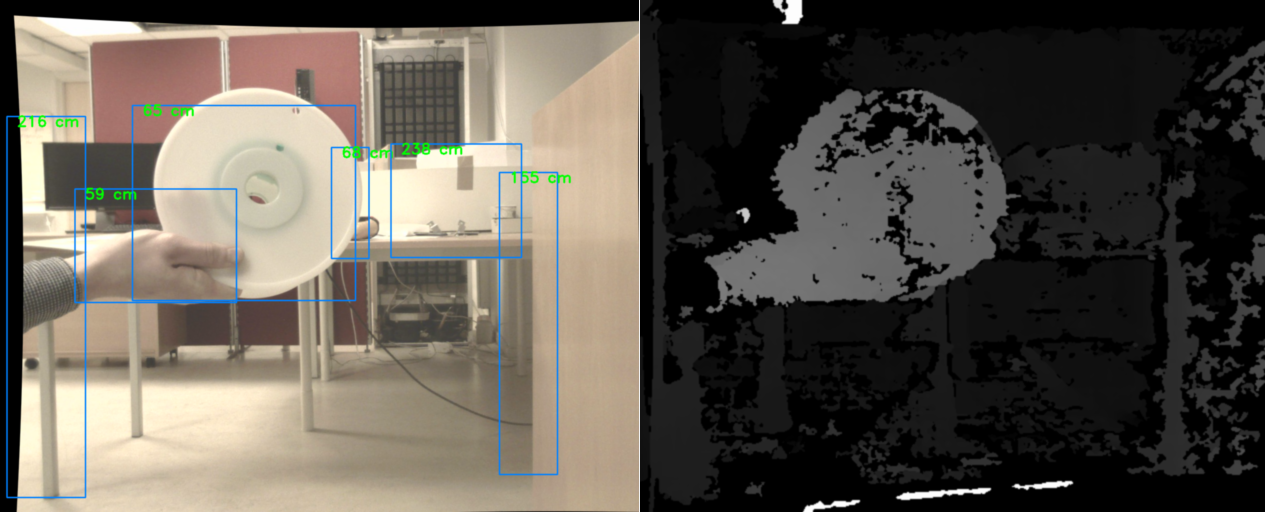
\includegraphics[width=1\textwidth]{rangeCalc}
	\caption{Obstruction detection in \textit{DepthFilter}.}
	\label{fig:rangeCalc}
\end{figure}

\subsection{Floor Filtering}

\begin{figure}
	\centering
	\begin{subfigure}[b]{0.48\textwidth}
		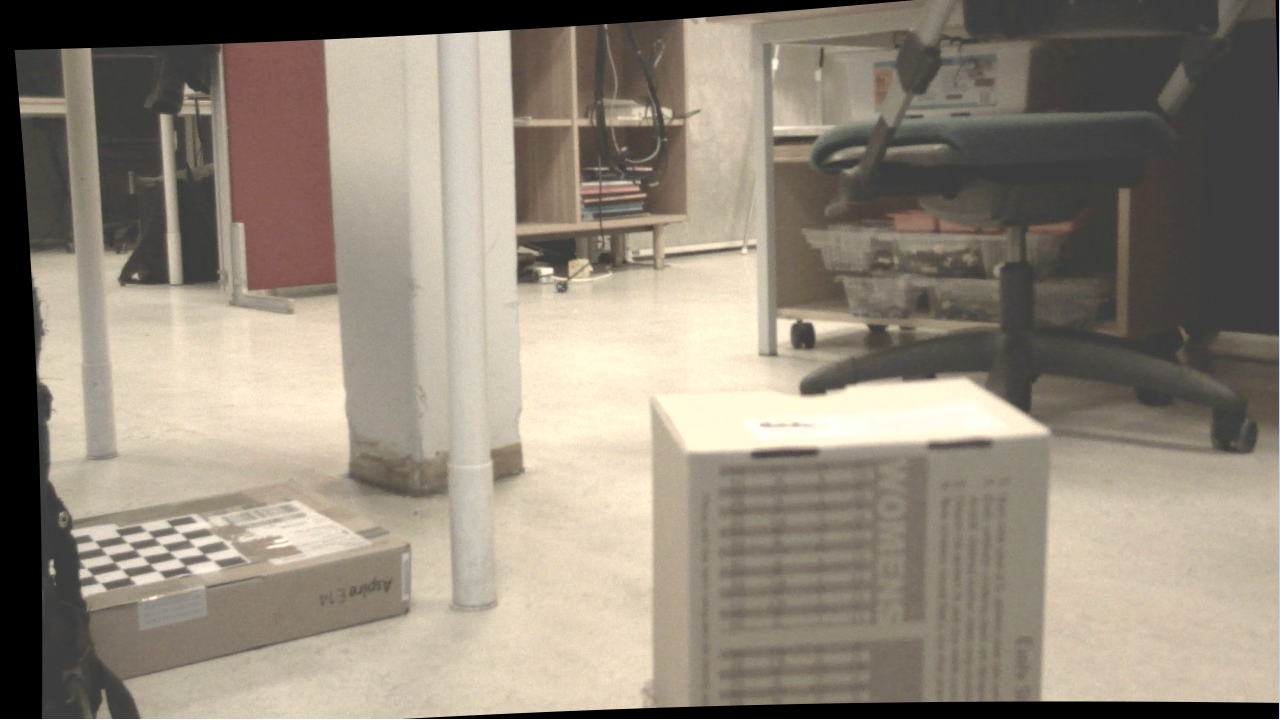
\includegraphics[width=\textwidth]{OriginalExample}
		\caption{Left camera image.}
		\label{fig:OriginalExample2}
	\end{subfigure}
	\begin{subfigure}[b]{0.48\textwidth}
		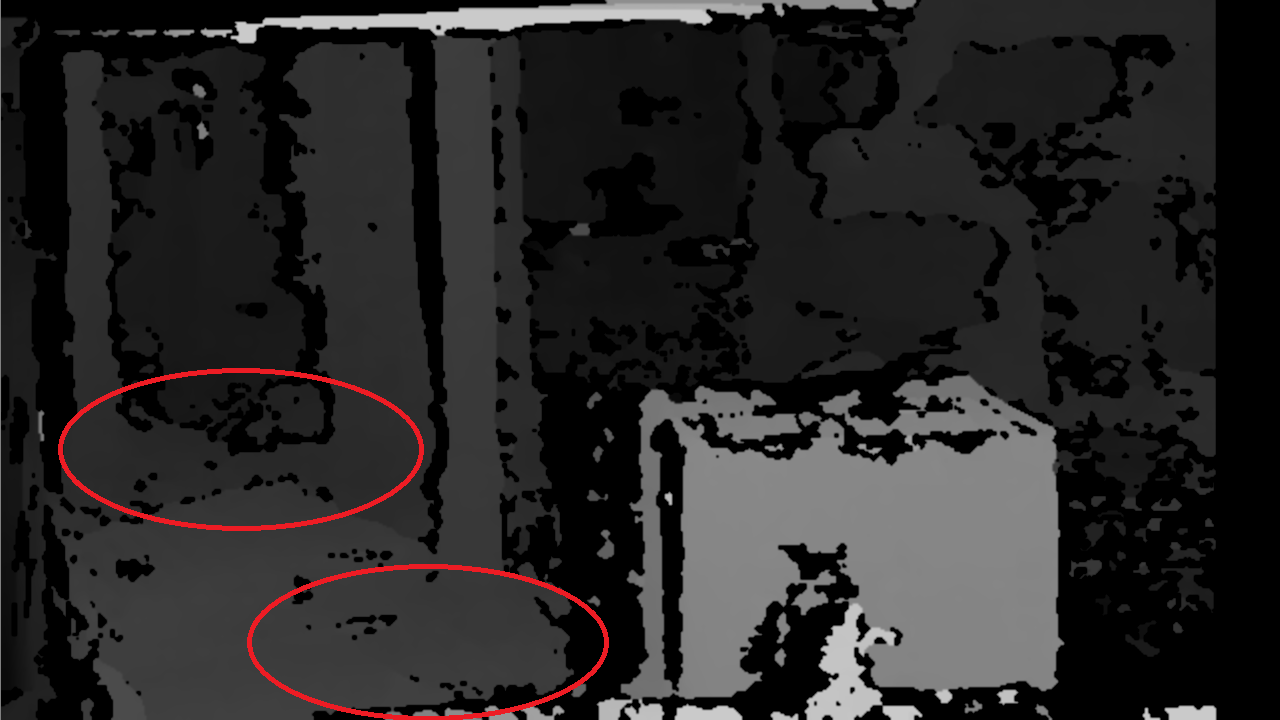
\includegraphics[width=\textwidth]{DispExampleWeakness}
		\caption{Disparity map.}
		\label{fig:DispExampleWeakness}
	\end{subfigure}
	\caption{\label{fig:distanceWeakness}The floor will have the same disparity value as two distict obstructions, thus making them appear as a single obstruction.}
\end{figure}

\begin{figure}
	\centering
	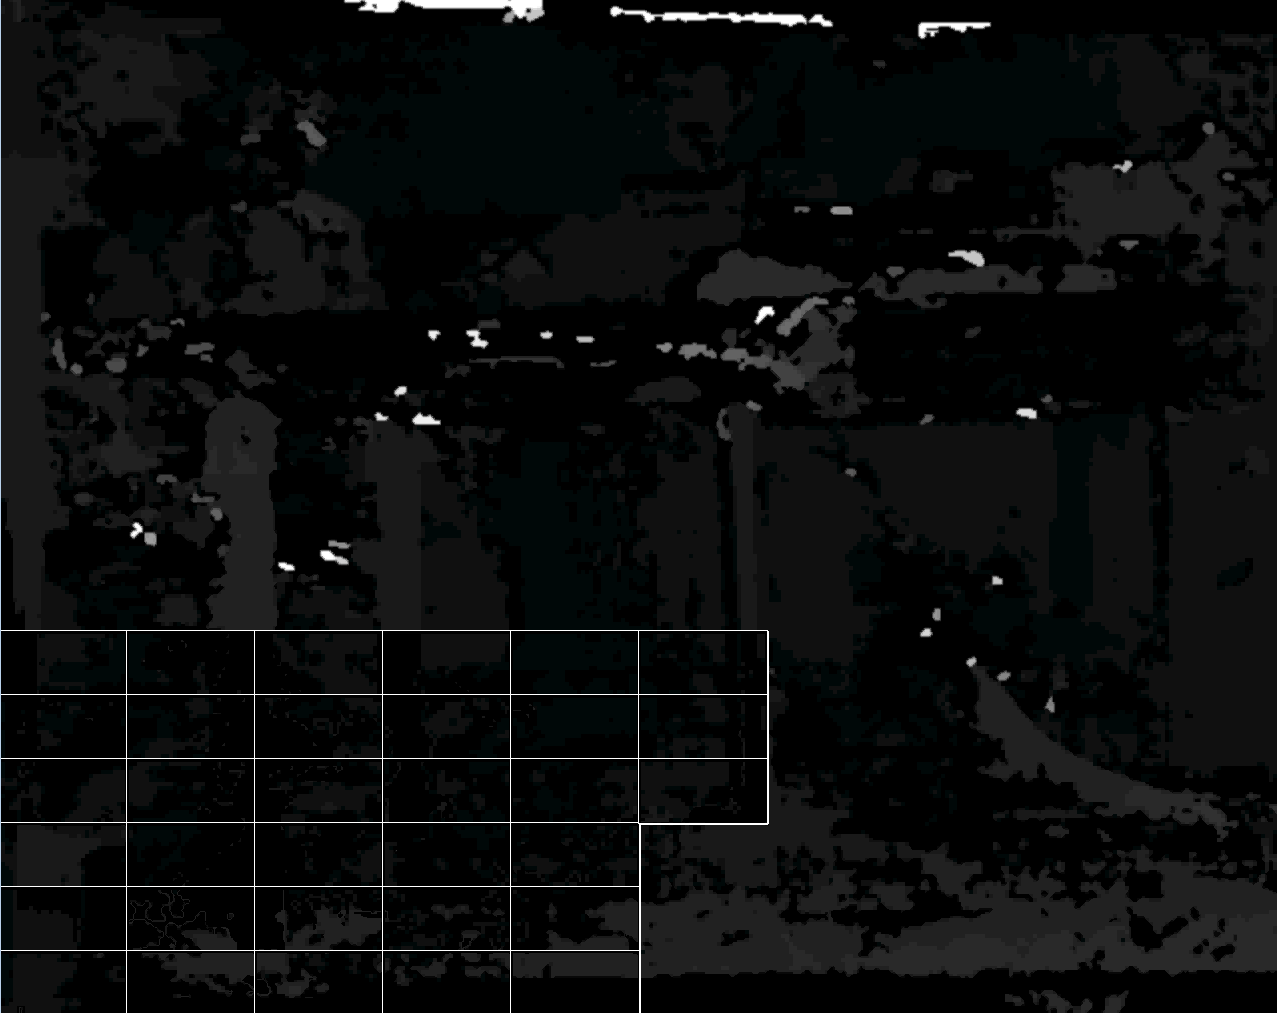
\includegraphics[width=1\textwidth]{floorFilter}
	\caption{Floor filtering in progress.}
	\label{fig:floorFilter}
\end{figure}
